%----------------------------------------------------------------------------------------
%	PACKAGES AND OTHER DOCUMENT CONFIGURATIONS
%----------------------------------------------------------------------------------------

\documentclass[paper=a4, fontsize=11pt]{scrartcl} % A4 paper and 11pt font size
\usepackage{graphicx} %For inserting pictures
\usepackage[T1]{fontenc} % Use 8-bit encoding that has 256 glyphs
\usepackage[english]{babel} % English language/hyphenation
\usepackage{amsmath,amsfonts,amsthm} % Math packages

%\allsectionsfont{\centering \normalfont\scshape} % Make all sections centered, the default font and small caps

\usepackage{fancyhdr} % Custom headers and footers
\pagestyle{fancyplain} % Makes all pages in the document conform to the custom headers and footers
\fancyhead{} % No page header - if you want one, create it in the same way as the footers below
\fancyfoot[L]{} % Empty left footer
\fancyfoot[C]{} % Empty center footer
\fancyfoot[R]{\thepage} % Page numbering for right footer
\renewcommand{\headrulewidth}{0pt} % Remove header underlines
\renewcommand{\footrulewidth}{0pt} % Remove footer underlines
\setlength{\headheight}{13.6pt} % Customize the height of the header

\numberwithin{equation}{section} % Number equations within sections (i.e. 1.1, 1.2, 2.1, 2.2 instead of 1, 2, 3, 4)
\numberwithin{figure}{section} % Number figures within sections (i.e. 1.1, 1.2, 2.1, 2.2 instead of 1, 2, 3, 4)
\numberwithin{table}{section} % Number tables within sections (i.e. 1.1, 1.2, 2.1, 2.2 instead of 1, 2, 3, 4)

\setlength\parindent{0pt} % Removes all indentation from paragraphs - comment this line for an assignment with lots of text
\DeclareGraphicsExtensions{.pdf,.png,.jpg}
\graphicspath{ {../images/} }
%----------------------------------------------------------------------------------------
%	TITLE SECTION
%----------------------------------------------------------------------------------------

\newcommand{\horrule}[1]{\rule{\linewidth}{#1}} % Create horizontal rule command with 1 argument of height

\title{	
\normalfont \normalsize 
\textsc{Dhirubhai Ambani Institute of Information and Communication Technology} \\ [25pt] % Your university, school and/or department name(s)
\horrule{0.5pt} \\[0.4cm] % Thin top horizontal rule
\huge Assignment 1 \\ % The assignment title
\horrule{2pt} \\[0.5cm] % Thick bottom horizontal rule
}

\author{Ganesh Iyer \\ 201311019 \\Developed using: Python(Using SimpleCV library)}

\date{\normalsize\today} % Today's date or a custom date

\begin{document}

\maketitle % Print the title

%----------------------------------------------------------------------------------------
%	PROBLEM 1
%----------------------------------------------------------------------------------------

\section{Image Resize}

In this problem I wrote a function that resizes an image to the given size \((M,N)\). We want to find a map such that for each \(P(x,y)\) belonging to \(I\), we get corresponding \(P'(x',y')\) in \(I'\). We define the notion of \textsl{Scaling Factor} \(S_x = M/ImageWidth\) and \(S_y = N/ImageHeight\). If \(I'\) were continuous we would have had \(x' = S_x*x\) and \(y' = S_y*y\) \(\forall x,y \in I\). In this exercise we achieved this effect by (1) Individually applying the transformation and then resampling it and (2)Using built-in functions for performing Affine Transformations.
%------------------------------------------------

\subsection{Nearest neighbor with pixel replication}

Nearest neighbor with pixel replication was implemented for this exercise. The transformation \(x' = S_x*x\) and \(y' = S_y*x\) was applied \(\forall x,y \in I\). We then resample the new coordinates \(x'\) and \(y'\) using  nearest neighbor method with pixel replication. 
Using nearest neighbor with pixel replication, We simply copy the intensity values, For all \((x', y')\) in \(I'\), to that of its nearest neighbor to the corresponding \((x,y)\) in \(I\). 

%------------------------------------------------

\subsubsection{Using Affine Transforms}

We can also scale images using the built-in functions available for performing affine transformations. These functions also provide a choice of the interpolating algorithm such as: Bilinear, Bicubic etc. We performed experiments with these algorithms, the results of which are reported in the subsequent sub-section. For scaling we used the following transformation matrix:

\(
  T = 
  \begin{pmatrix}
    S_x && 1 && 0 \\
    1 && S_y && 0 \\
    0 && 0 && 1
  \end{pmatrix}
\) 

\subsection{Results}
  \begin{figure}[h!]
    \centering
    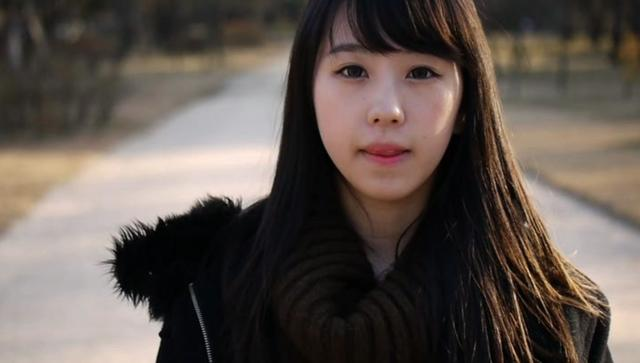
\includegraphics[clip,height=3cm]{1}
    \caption{Original image}
  \end{figure}

  \begin{figure}[h!]   
    \centering
    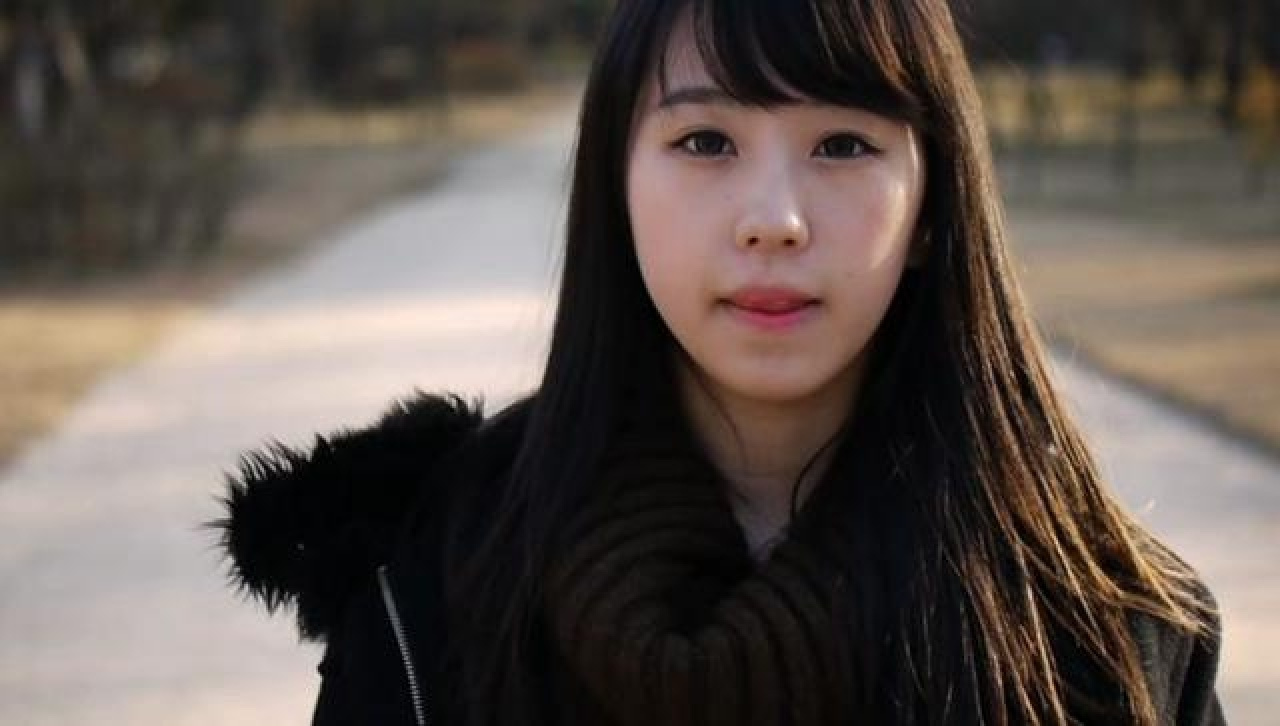
\includegraphics[clip,height=3cm]{resized2x}
    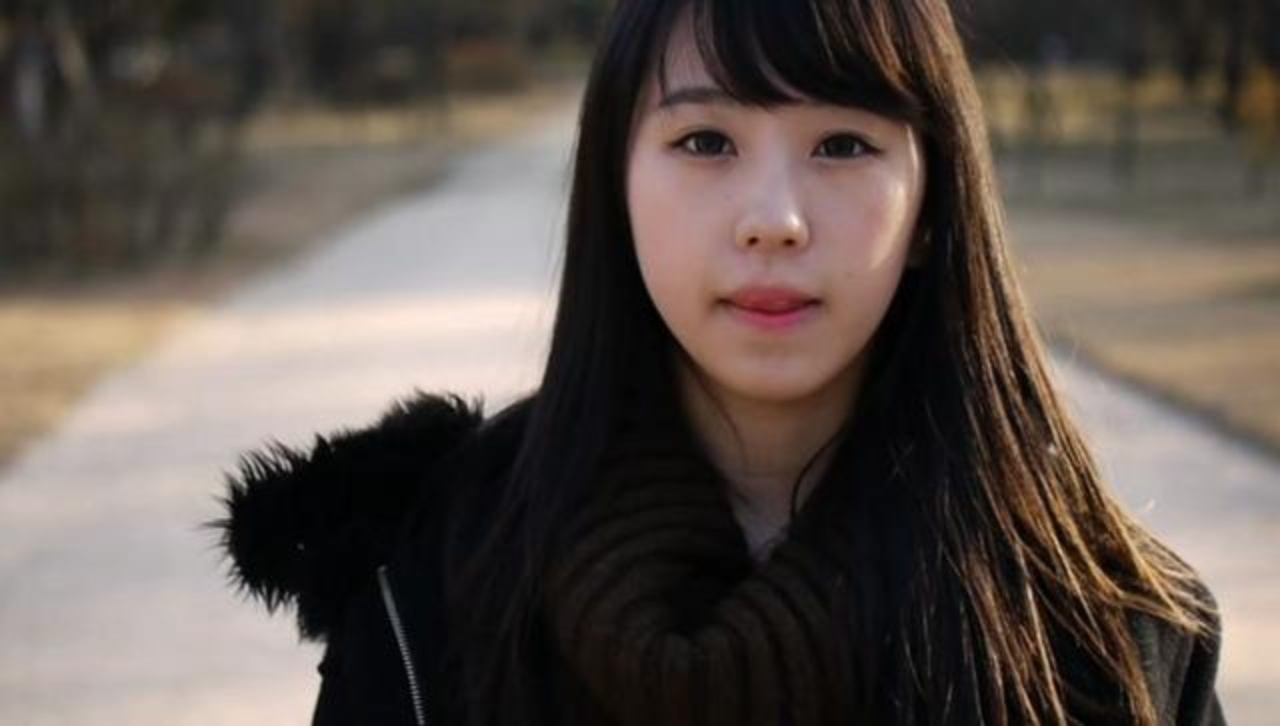
\includegraphics[clip,height=3cm]{scvresized2x}
    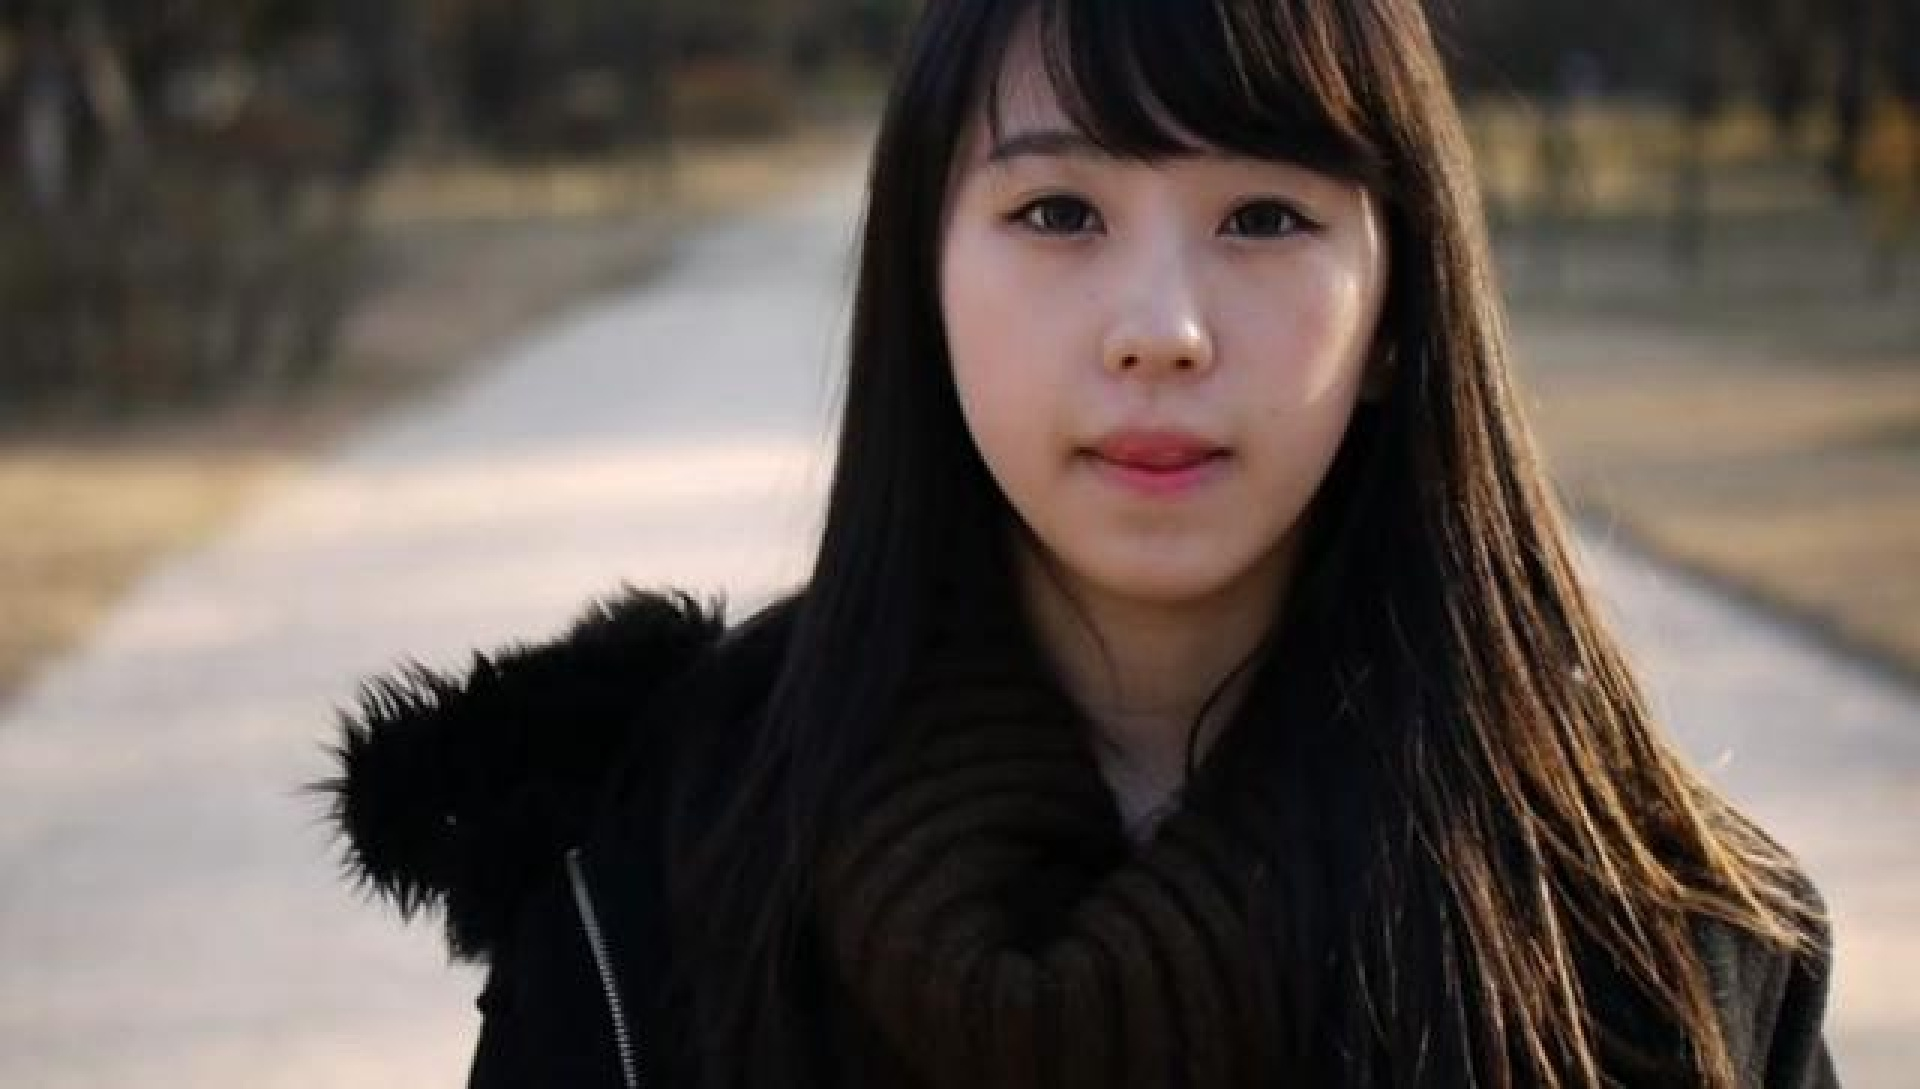
\includegraphics[clip,height=3cm]{resized3x}
    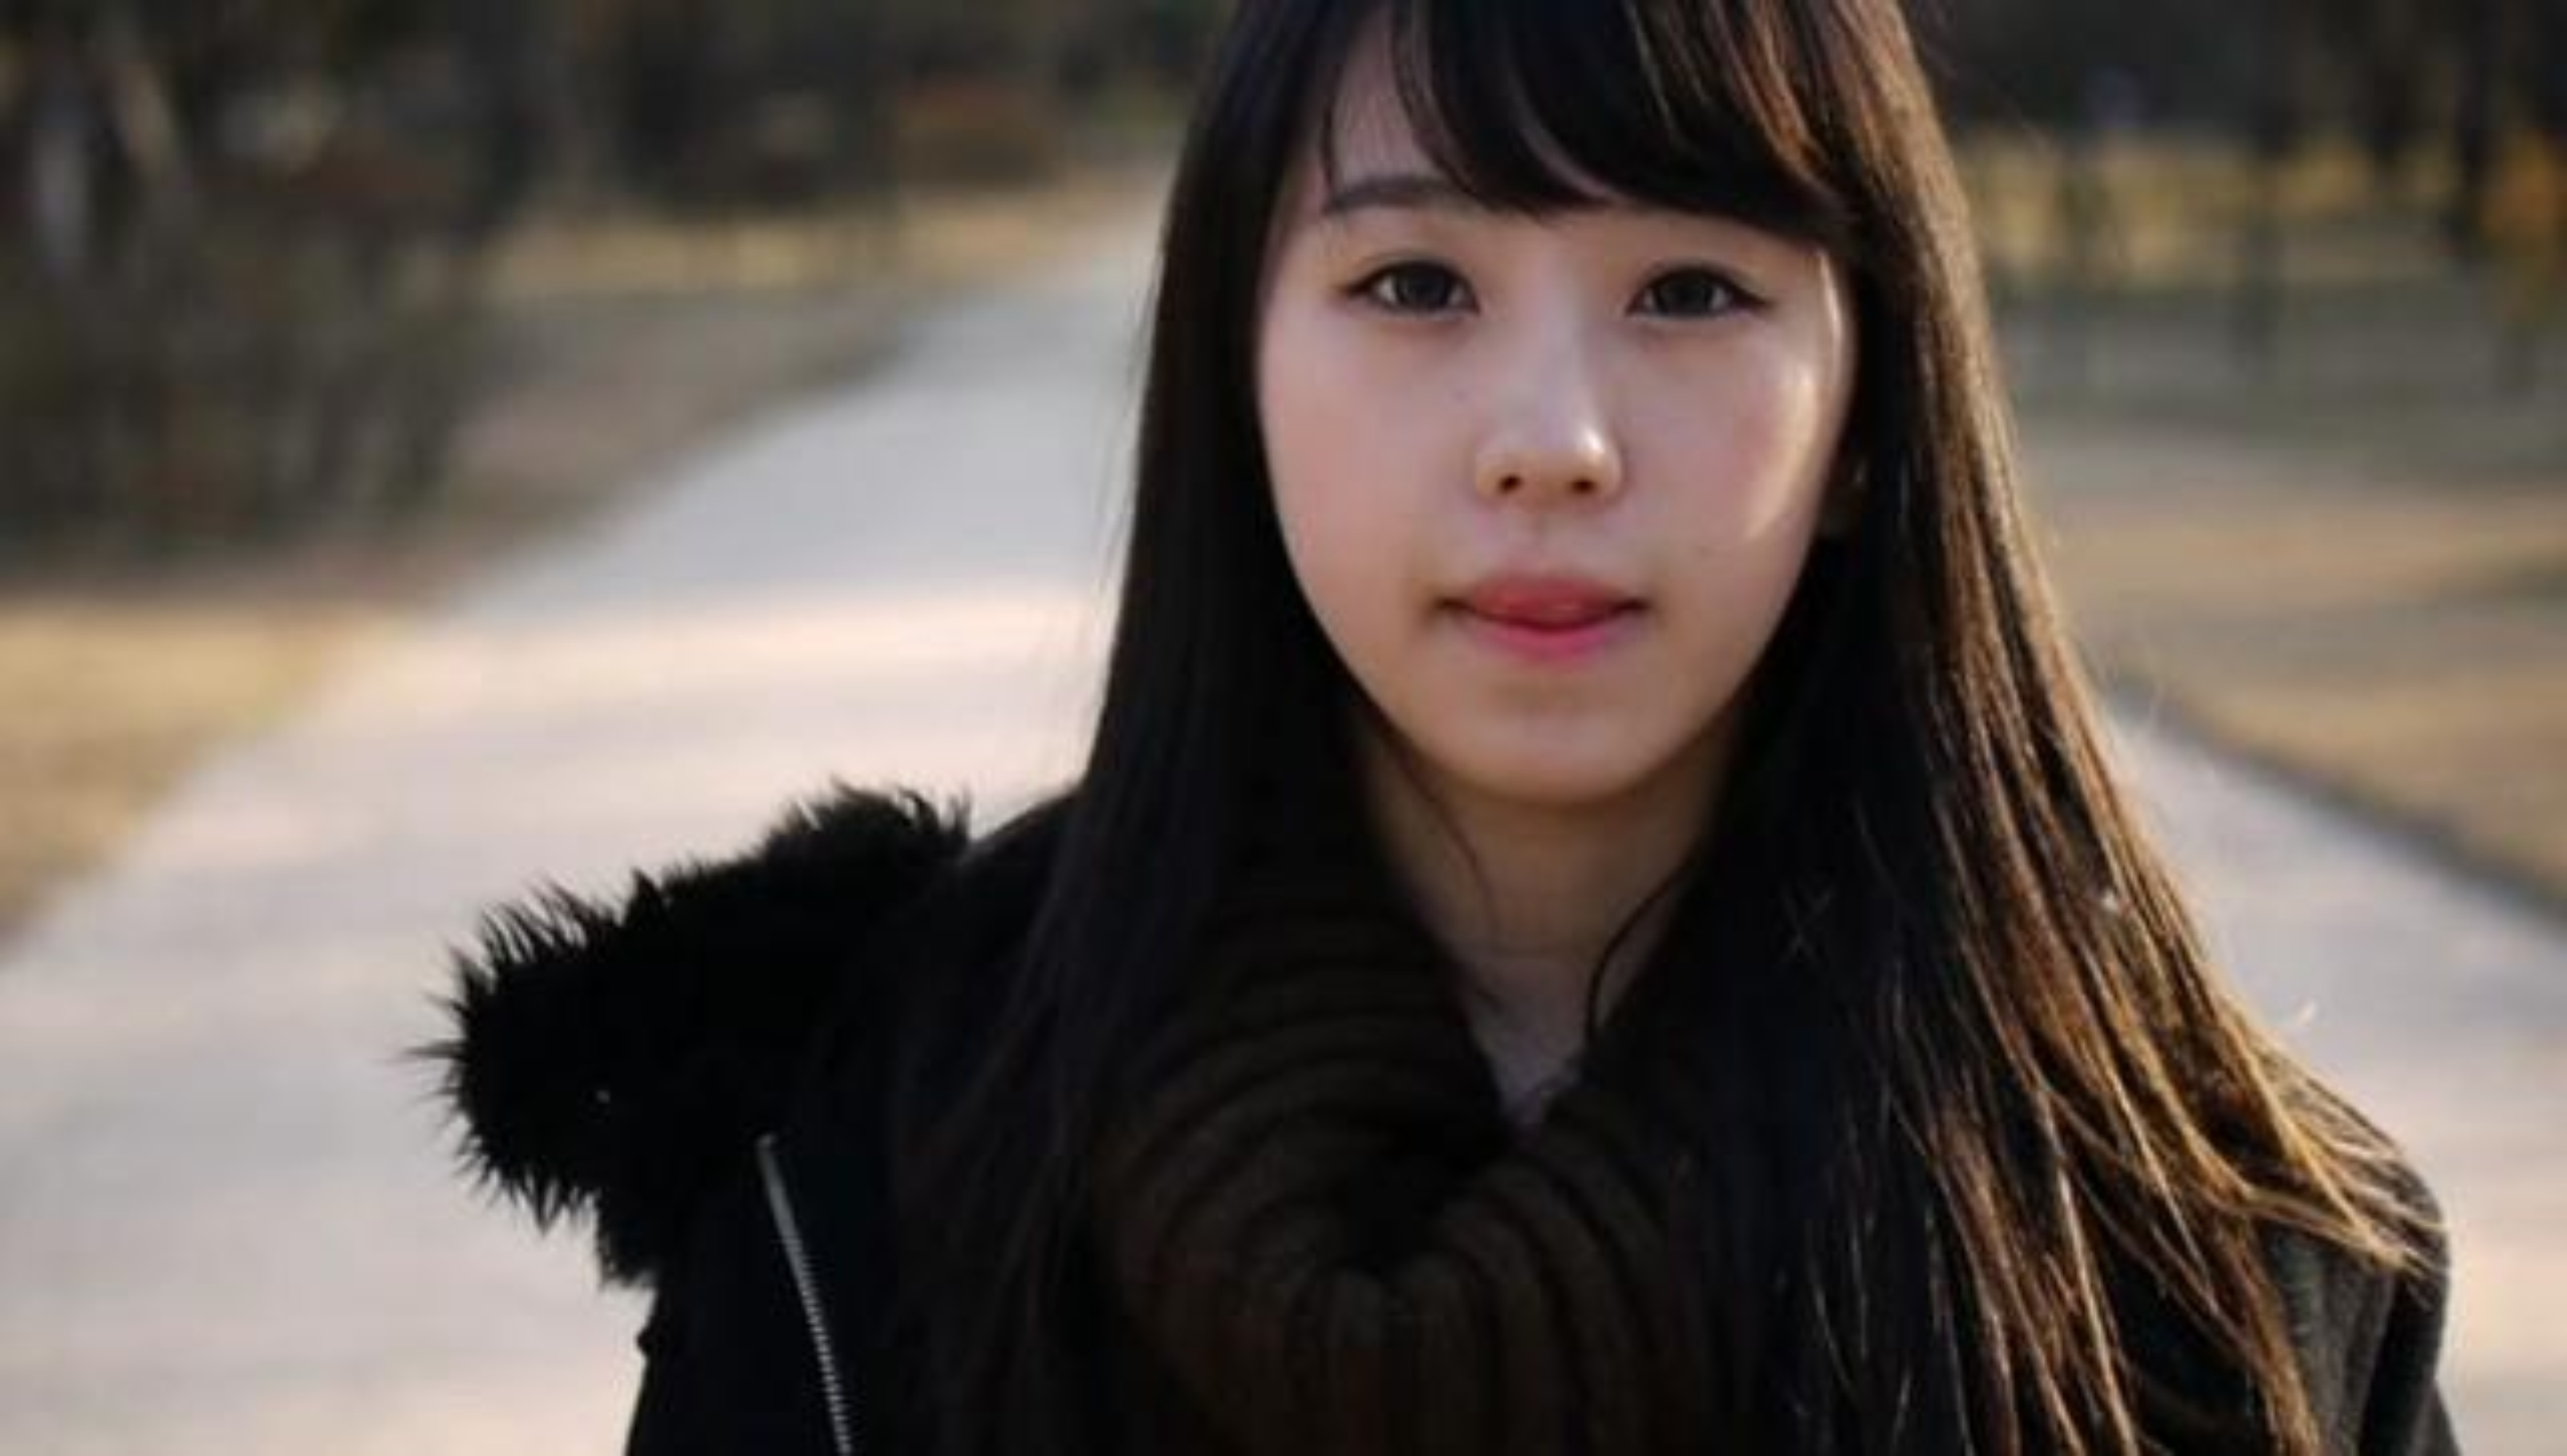
\includegraphics[clip,height=3cm]{scvresized3x}
    \caption{Clockwise from topleft: Image scaled 2 times using myresize, scaled 2x using built-in function, 3x using myresize, 3x using built-in function. Please note these results have been resized again to fit the document. For seeing the original effect please refer to the images folder}
  \end{figure}
  
%----------------------------------------------------------------------------------------
%	PROBLEM 2
%----------------------------------------------------------------------------------------

\section{Image rotation}

In this exercise, given an input image(\(I)\) and angle(\(\theta\)), we had to generate an output Image(\(I')\)) which is the result of rotating \(I\) by an angle \(\theta\) about the center of the image. For this we used an affine transformation, with transformation matrix:

\(
  T = 
  \begin{pmatrix}
    \cos(\theta) && \sin(\theta) && c_x(1-\cos(\theta)) - c_y(\sin(\theta)) \\
    -\sin(\theta) && \cos(\theta) && c_y(1 - \cos(\theta)) + c_x(\sin(\theta)) \\
    0 && 0 && 1
  \end{pmatrix}
\) 
where \((c_x,c_y)\) are the coordinates of the center of the Image.\\
We use the Bicubic interpolation with this transformation


\subsection{Results}
  \begin{figure}[h!]   
    \centering
    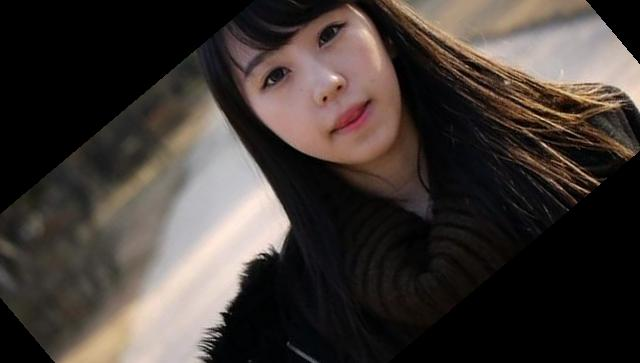
\includegraphics[clip,height=3cm]{rotate40}
    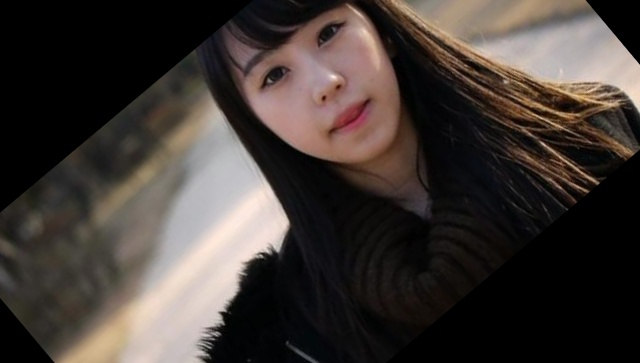
\includegraphics[clip,height=3cm]{scvrotate40}
    \caption{Image rotated at an angle 40 degrees using myrotate, Image rotated at an angle 40 degrees using built-in function}
   \end{figure}
%----------------------------------------------------------------------------------------

%----------------------------------------------------------------------------------------
%	PROBLEM 3
%----------------------------------------------------------------------------------------

\section{Affine Trasformation}

Given the corner vectors of input image, \(p_{in}^k = (x_k,y_k,1), 0 \leq k \leq 3\). We want to map this to the region enclosed by \(p_{op}^k = (u_k,v_k,1), 0 \leq k \leq 3 \). In this exercise we derive the number of such corner points that are required to uniquely define the affine transformation. Also we develop a function to generate the transformation matrix from the required number of points.

%------------------------------------------------

\subsection{Number of points required to define the affine transformation}

A generic affine transformation matrix is of the form
\(
  T = 
  \begin{pmatrix}
    a && b && c\\
    d && e && f\\
    0 && 0 && 1
  \end{pmatrix}
\) 

Now from \(p_{op}^k = T*p_{in}^k\)\\
We have equations of the form \\
\(u_i = ax_i + by_i + c\) and\\
\(v_i = dx_i + ey_i + f\)\\
Both of them are equations with 3 variables thus we just need 3 points to solve this system of equations. Thus only 3 corner points are required to determine the transformation.

Also for a unique solution
\(
  \delta = 
  \begin{vmatrix}
    x_1 && y_1 && 1 \\
    x_2 && y_2 && 1 \\
    0 && 0 && 1
  \end{vmatrix} 
  \neq 0
\)



\subsection{Function to generate the transformation matrix}

Given 3 corner points \(p_{in}^k = (x_k,y_k,1), 0 \leq k \leq 2\) and their corresponding output points \(p_{out}^k = (u_k,v_k,1), 0 \leq k \leq 2\). We need to find values of \(a,b,c,d,e,f\) to find out the transformation matrix. We can represent the system of equations in matrix form as:

\(Ax = u\)

where \( A =
        \begin{pmatrix}
          x_1 && y_1 && 1\\
          x_2 && y_2 && 1\\
          x_3 && y_3 && 1  
        \end{pmatrix}
      \) , \(x = \begin{pmatrix} a\\ b\\ c \end{pmatrix}\) and \(u = \begin{pmatrix} u_1\\ u_2\\ u_3 \end{pmatrix}\)
Solving this using Cramer's rule we get values of \(a, b\) and \(c\)
Similary we can solve
\(Bx = v\) to find \(e,f\) and \(g\)

%----------------------------------------------------------------------------------------
%	PROBLEM 4 
%----------------------------------------------------------------------------------------

\section{Fisheye effect}

In this exercise we generated images with Fisheye effect. We apply the following transformation to each pixel \((x,y)\) in the image

\(x_d = x_c + \frac{x - x_c}{1 + k(\frac{r}{r_{max}}}) \)\\
\(y_d = y_c + \frac{y - y_c}{1 + k(\frac{r}{r_{max}}}) \)

Where \((x_d, y_d), (x_c, y_c)\) are the coordinates of distorted image and original Image respectively, \((x_c,y_c)\) are the coordinates of distortion center(which is the image center), \(r\) is the Eucledian distance between \((x_d, y_d)\) and \((x_c, y_c)\) and \(k \in \mathbb{R}\) .
%------------------------------------------------

\subsection{Results}
  \begin {figure}[h!]
    \centering
    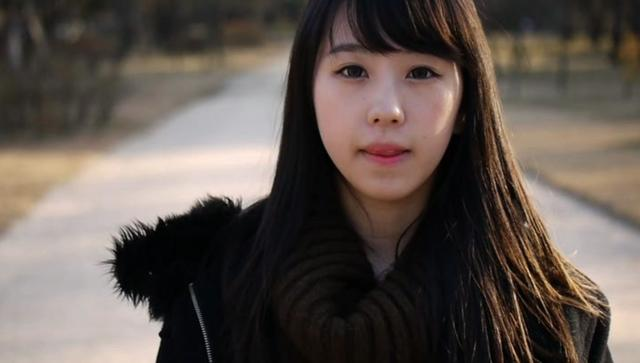
\includegraphics[clip,height=3cm]{1}
    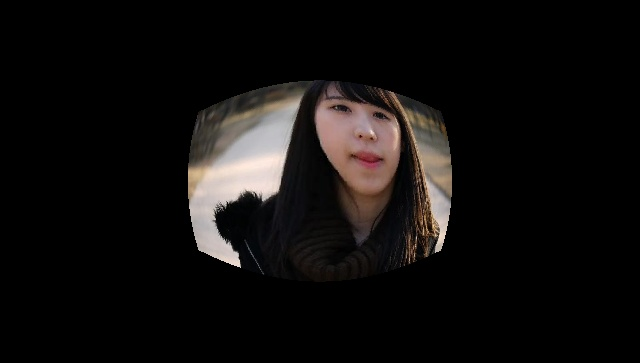
\includegraphics[clip,height=3cm]{Fisheye01}
    \caption {Fisheye effect with k=0.1}
  \end{figure}
%----------------------------------------------------------------------------------------

\end{document}
